\chapter{The Design and Development of the Immotion Exergame}\label{chapter:implementation}

This chapter outlines the design and development of the Immotion exergame for warm up routine guidance and motivation. We begin this chapter with the description of the design methodology used for the development. For the purpose of this thesis, an iterative and prototype driven, user centered design methodology has been adopted. After the methodology has been introduced, we continue with the in depth discussion of each individual development phase. Our main focus is placed on the last two stages of the development process in which we develop the prototype and the final version of our exergame solution, and evaluate them utilizing various qualitative evaluation methods. During all the development phases, the particular needs of individuals who engage in physical (sports) activities but rarely or never warm up prior to them have been taken into account and gathered through the adopted design process in order to make an adequate exergame for warm up guidance and motivation. %We chose the \textit{Spiral model}s as our chosen exergame development model.  

\section{Overview of User Centered Design}
\gls{ucd} represents \textit{a user interface design process} that puts its focus on usability goals, explicit understanding of users, environment, and tasks to be performed []. Moreover, it is an iterative process, where design and evaluation phases are included from the first stage of the development, that addresses the whole user experience, and is driven and refined by user-centered evaluation. %Shawn Lawton Henry and Mary Martinson, Accessibility in User-Centered Design + https://www.w3.org/WAI/redesign/ucd + https://www.usability.gov/what-and-why/user-centered-design.html
Adopted from \cite{userCenteredDesign}, the following are the general and advised phases of the \acrshort{ucd} process:
\begin{itemize}
\item \textit{Specify the context of use}. Identify future users of the solution, the intended purpose of usage, and the conditions under which the solution will be used.
\item \textit{Specify requirements}. Identify user goals that must be met in order for the solution success.
\item \textit{Create design solutions}. Done in stages, building from a rough concept to a complete and final design.
\item \textit{Evaluate designs}. Evaluation should be performed through usability testing with actual users.
\end{itemize}
Even though being a relatively new field, exergame developers often indicate the relevance of including the players in the design process and point out the benefits of adopting \acrshort{ucd} in exergames development. In their study on exergame design for elderly users, Gerling and Masuch recommend and utilize \acrshort{ucd} for developing exergames for an elderly audience []. Researchers in [] also take advantage of \acrshort{ucd} in their year long study whilst developing action-oriented exergames for children with cerebral palsy. As showed that \acrshort{ucd} can be used for designing effective exergames for specific target demographic, we also adopt this approach in the development of our exergame solution for warm up guidance and motivation.
\section{The Context of Use}
There exist solutions designed to encourage physical activity. These solutions are mainly intended to be used for home and in-door workout activities. Many of them offer multitudes of predefined exercise programs and also make it easy to create a fully customized workout plan that are suited for individual's needs and abilities [cite wifit and stuf]. However, in our research, we found no available solutions that focus solely on the warm up routine as a preparatory activity before physically more demanding exercise. Taking this into account, as well as the fact that warm up routines are crucial part of any sports activity \cite{bishop2003warm1,shellock1985warming} although often avoided by multitude of athletes \cite{fradkin2006does}, with the Immotion exergame we chose to tackle exactly this issue. We design and develop our exergame to be used as a warm up guidance and motivation tool. That is, our exergame is intended to be used in gyms and fitness centers before any arduous sports activity. Additionally, we target individuals, above all amateur athletes, who do not know how to perform a proper warm up routine before the subsequent sport activity. Lastly, we design our exergame so the movements required to be executed by the player are intuitive and do not require additional explanation nor previous exercise knowledge. \pagebreak
\section{Overview of the Development Phases}
The development of the Immotion exergame consisted of three primary phases which are according to the well accepted \acrshort{ucd} development phases outlined in the previous section and depicted in Figure \ref{fig:iterations}: 
\begin{itemize}
\item Requirements gathering 
\item First prototype development with user evaluation
\item Final exergame development with further user evaluation
\end{itemize}
In the following sections, each iteration presented in \textit{Development} slice and the \textit{Requirement Gathering} iteration of the \textit{Planning} slice depicted in Figure \ref{fig:iterations} will be further detailed. 
\begin{figure}[h]
    \centering
    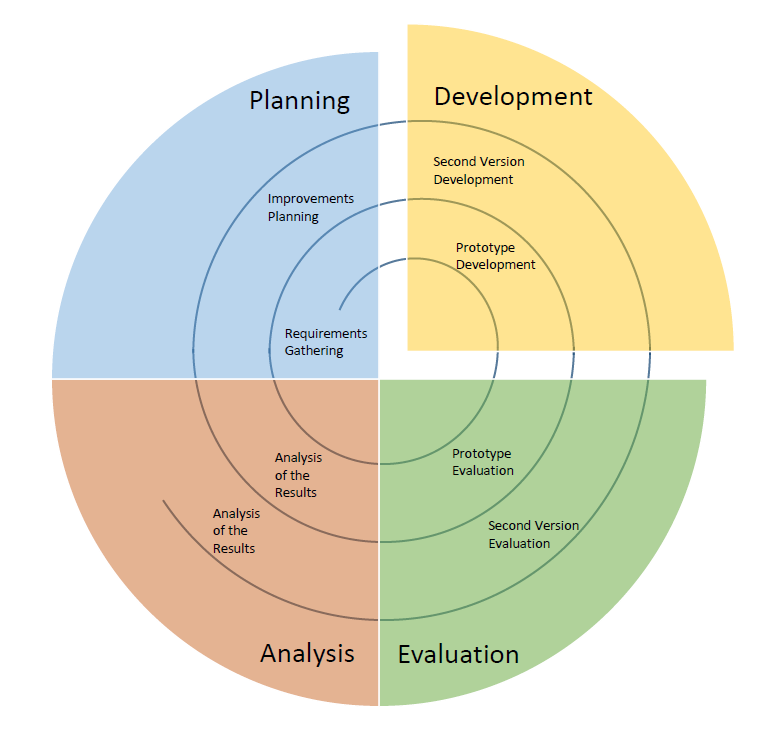
\includegraphics[width=0.9\textwidth]{iterations}
    \caption{Overview of the development iterations}
    \label{fig:iterations}
\end{figure}
\subsection{Requirements Gathering}
This iteration was an exploratory step that justified the development and identified the currently available solutions in the domain of exergames for warm up before sports activities. This was achieved through initial literature review related to exergame, gamification, and motivational psychology which identified the most important areas to be addressed when developing gamified solution in the given context. Furthermore, in order to design an enjoyable exergame solution, several warm up and sports related requirements needed to be considered too. Having this in mind, sports and fitness related literature have been reviewed as well. Particular attention has been put on those warm up exercises that could hypothetically help in injury prevention and improve performance. \\As previously pointed out, our exergame is meant to be used in gym or fitness centers before physically demanding sports activities. Hence, the movements required in the game should be those that increase core body temperature, blood flow, and prepare the body for the subsequent exercise. In addition, we had to take into account certain constraints and requirements when selecting these movements. Some of the them were as follows:
\begin{itemize}
\item Movements needed to be easily detectable by only one Kinect device.
\item Movements should be easy enough to be correctly performed without any prior knowledge of the movement or exercise.
\item Only movements that can be executed without additional equipment should be considered.   
\item Only movements recommended for the general warm up routines outlined in sports related literature and suggested by experts should be considered.
\item The duration of the exergame guided warm up routine should correspond to the warm up duration suggested by sports literature and experts.
\end{itemize}
%http://assets.ngin.com/attachments/document/0035/1162/FIFA_11__EXERCISES.pdf
%https://www.kort.com/uploadedFiles/KORT/Content/Services/Sports_Medicine/Concussion_Management/FIFA-the-11-Booklet.pdf
Since no well documented and medically supported warm up programmes for workout routines were found,  the required movements were adopted from the 
\gls{fifa} \cite{fifa} warm up programme which mostly focuses on core and leg strength, balance, and agility. These programmes were shown to have significant impact on injury reduction in football players and can lead to improvements in thigh muscle strength, jump height, and sprint speed []. %https://www.ncbi.nlm.nih.gov/pmc/articles/PMC4245655/
Based on the mentioned warm up programs review, the previously listed requirements, and hardware restrictions outlined, the following movements were found to be suitable for the prototype solution: 
\begin{itemize}
\item jump right,
\item jump left,
\item jump up, and
\item squat.
\end{itemize}
After the requirements were specified and the required movements selected, we continued with the prototype development phase.
\subsection{Prototype Development}
This section outlines the development of the prototype version of the exergame for warm up guidance and motivation before sports activities. Our primary goal was to develop a working version of the exergame that can process movements in real time in order to guide users through the warm up routine and, presumably, immerses the participants sufficiently so that their focus is shifted from the discomfort and exertion of the exercise towards the enjoyment of the experience. The prototype was developed as a scaled down version of our planned final solution. With the prototype, we aimed to learn more about the problem, possible target groups, and explore the most suitable design and implementation techniques that could be used during the exergame development process. 
\subsubsection{Game Description}
The Immotion exergame was created using Unity 5.6 game development platform developed by Unity Technologies []. Players' movements were captured and processed with Kinect for Xbox One (2.0 2013) motion sensing input devices by Microsoft []. The game engine was run on XX [] and projected on a wall using XX projector. In figure \ref{fig:hs} we outline the relationship of the game, software, and hardware equipment.\\
\begin{figure}[h]
    \centering
    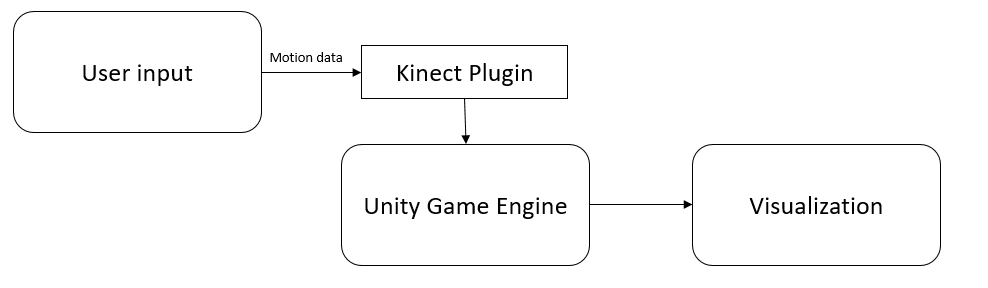
\includegraphics[width=\textwidth]{hardware_software}
    \caption{Hardware and Software supporting the prototype exergame}
    \label{fig:hs}
\end{figure}\\
For the prototype version of the exergame, a game scenario that is similar to \textit{Subway Surfers} [] and \textit{Temple Run} [] games was implemented. In these games, the player controls the character that is on a track and needs to move left, right or jump up in order to avoid obstacles and collect points. In our solution, the player controlled the character by doing a set of movements, which were tracked in real time with a Microsoft Kinect device. In-game obstacles (e.i. walls or boxes) and coins were positioned in a way that the player was required to perform a specific movement in order to avoid the obstacle or collect a coin. By collecting coins the overall player's score was increased. Contrarily, by hitting an obstacle, the overall player's score was decreased. By placing the obstacle and coins in a specific position, our intention was to indirectly promote exercise through the gameplay of repeatedly performing warm up related movements chosen during previous development phases. Figure \ref{fig:prototypeUsage} depicts the usage of the prototype version of the Immotion exergame during one of our final tests.
\begin{figure}[h]
    \centering
    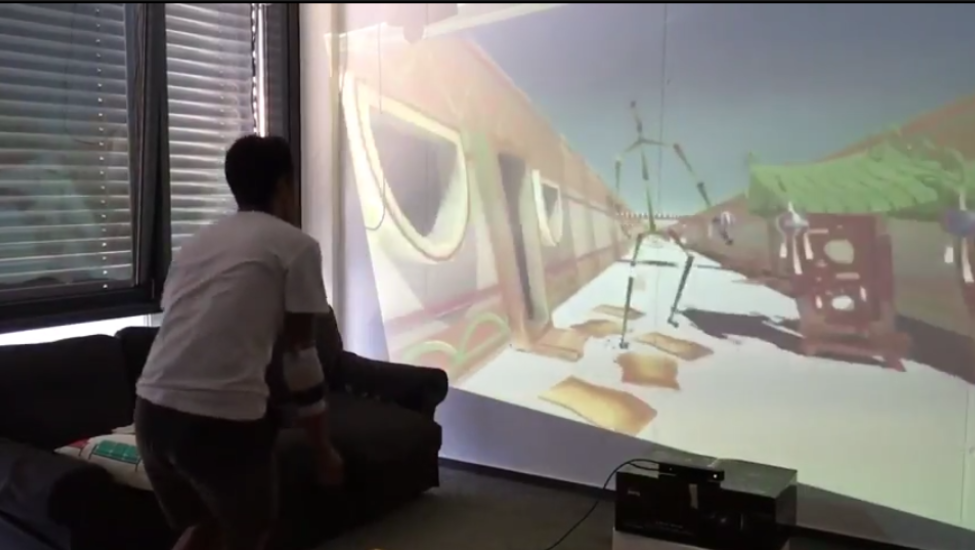
\includegraphics[width=\textwidth]{prototypeUsage}
    \caption{Interacting with the prototype version of the Immotion exergame}
    \label{fig:prototypeUsage}
\end{figure}\\ \\
Next, the main gamification elements that are incorporated into our exergame are further discussed.
\subsubsection{Gamification Elements}
In order to create an immersive game environment that will shift users' focus from the exertion of the exercise, we also employ few game \textit{mechanics}.  Werbach and Hunter report that mechanics provide the ''\textit{basic processes that drive the action forward and generate
player engagement}'' \cite{werbach2012win}. For the prototype version of the Immotion exergame, the most important mechanics was \textit{Feedback}.

\subsubsection{Feedback}
As pointed out in Chapter \ref{chapter:relatedwork}, feedback have been shown to influence and improve autonomy and, hence, the intrinsic motivation of individuals. %[Ryan 2006]
Warbach and Hunter argue that giving unanticipated, informal feedback or support about the player's progress can provoke increased intrinsic motivation and autonomy \cite{werbach2012win}. They further outline that gamification components represent specific examples and ways for doing the higher level things that gamification mechanics and dynamics represent. In the prototype version of the exergame, the player receives the feedback using different gamification components that will be further detailed.

\subsubsection{Gamification Components}
\paragraph{Points}
According to Zichermann and Cunningham \cite{zichermann2011gamification} points are ``\textit{an absolute requirement for all gamified systems}'', because they can serve a wide range of purposes. One of the most obvious is for keeping a score and evaluate progress of the user. However, they can serve as a powerful extrinsic motivator for player types that enjoy collecting points, like \textit{Killers} or \textit{Achievers}. In the prototype version of the exergame, the player could earn points by collecting coins and lose them by hitting an obstacle. How much points could the player earn or lose by each action is presented in Figure \ref{fig:points}.\\
\begin{figure}[h]
    \centering
    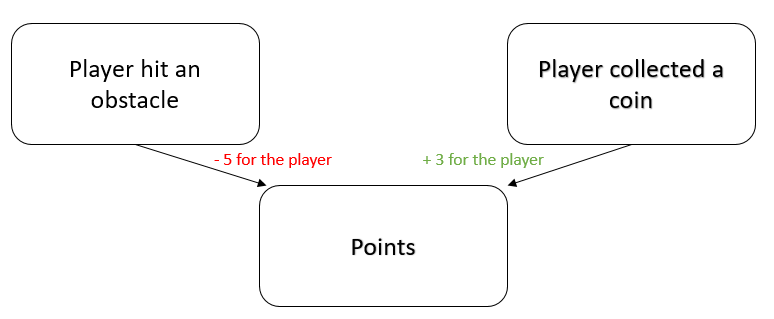
\includegraphics[width=\textwidth]{points}
    \caption{Earning and loosing point in the prototype version of the exergame}
    \label{fig:points}
\end{figure}\\
As per Figure \ref{fig:points}, the player could earn 3 points by collecting a coin. Contrarily, the player could lose 5 points if hit by an obstacle. In order to avoid hitting an obstacle or collect a coin, a movement was required to be performed by the player. Consequentially, the player was guided through the warm up routine without even realizing it. In the course of the game, the player's current score was displayed in the right corner. That way, the player had constant overview of her progress.  
\paragraph{Avatar}
In the prototype version of the game we used a simplistic avatar which players controlled by performing the movements in front of the Kinect sensor. The main purpose of the avatar was to correctly replicate player's movements. By doing so, the player got a real time feedback on how the movement was performed. The avatar that was utilized for the prototype version is presented in Figure \ref{fig:avatar_prototype}.\\
\begin{figure}[h]
    \centering
    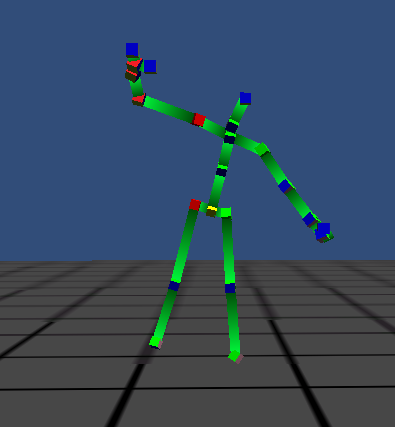
\includegraphics[width=0.6\textwidth]{avatar_prototype}
    \caption{The avatar used in the prototype game.}
    \label{fig:avatar_prototype}
\end{figure}
\paragraph{Visual Feedback}
Even though cannot be counted among gamification components, for the purpose of giving players the necessary feedback, we introduced additional visual components. The player was informed when a game obstacle is hit by the avatar. This was done by adding red overlay to the scene every time event of this kind occurred. This informed the player that the last movement was not successful, and deducted points from players overall score.
\paragraph{Audio Feedback}
Similarly to previous component, audio cues were introduced to inform the player of success or failure of the performed movement. In case the player managed to collect a coin successfully, a sound comparable to the one heard when collecting a coin in many video games is played. Contrarily, a crashing sound was played on failure when the player hit an obstacle. The volume of the sounds played on success or failure were balanced as much as possible so that they were distinct enough but not disturbing to the player of the exergame.
\subsection{Game Scenes}
Figure \ref{fig:prototype} shows the scenes from the prototype version of the exergame. The prototype has been pilot-tested with few student volunteers. During the pilot testing, the interaction with the exergame has been recorded for further analysis and evaluation [link yt]. 
\begin{figure}[h]
    \centering
    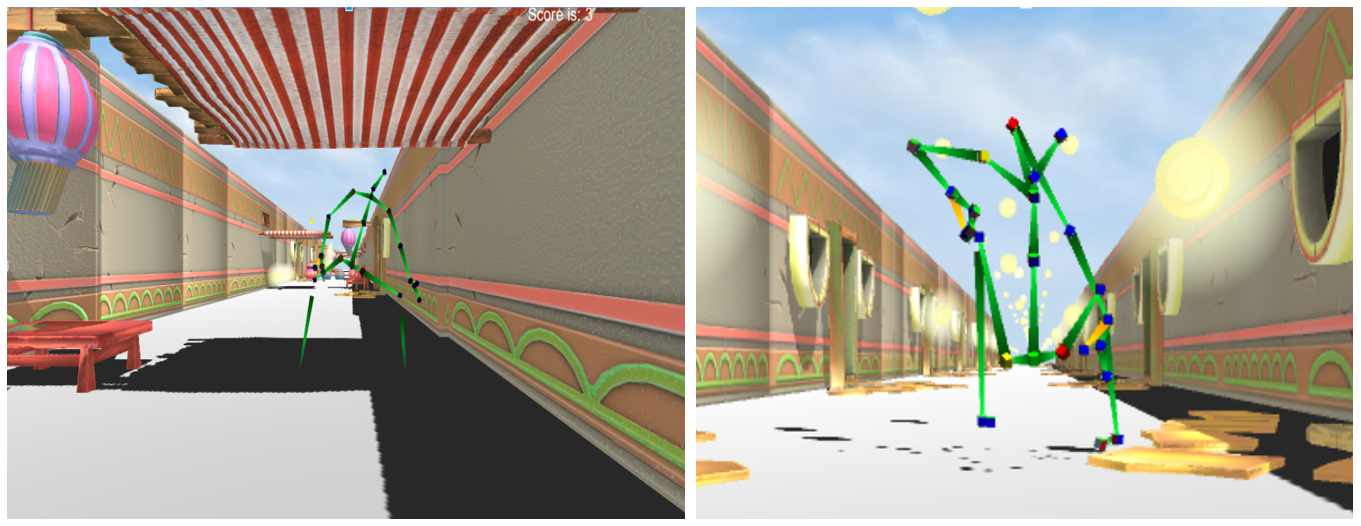
\includegraphics[width=\textwidth]{prototype}
    \caption{Game scenes from the prototype version of the exergame}
    \label{fig:prototype}
\end{figure}\\
In the next chapter, we present the evaluation of the prototype exergame. Through a survey, we evaluated which features of the gamified system are appreciated the most and which the least, and hence can be removed or improved in the final exergame release.